\begin{figure}[ht]
\centering
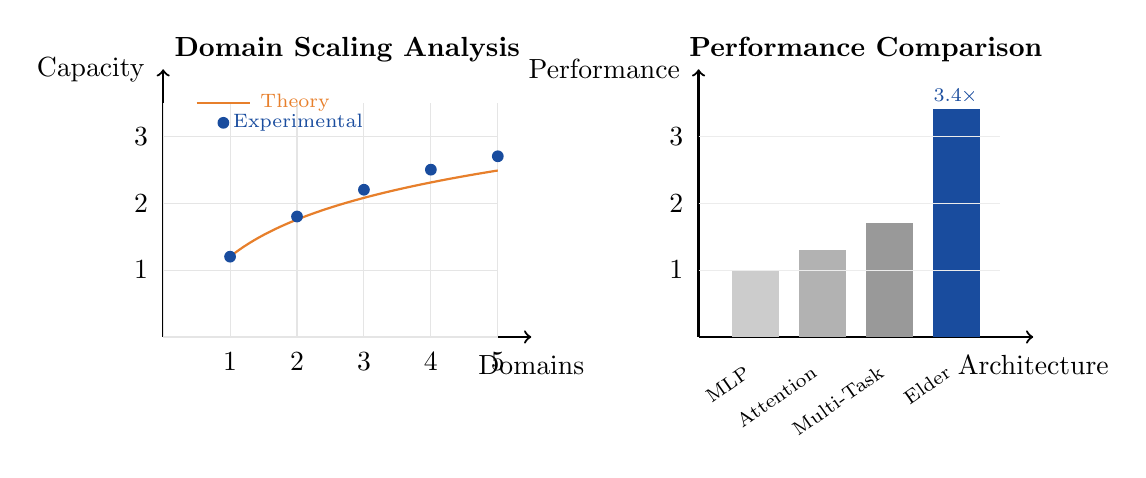
\begin{tikzpicture}[scale=0.85]
    % Define colors
    \definecolor{elderblue}{RGB}{25,76,158}
    \definecolor{elderorange}{RGB}{231,127,43}
    
    % Simplified Domain Scaling Plot
    \begin{scope}[shift={(0,0)}]
        % Title with more space
        \node[font=\normalsize\bfseries] at (2.75,4.3) {Domain Scaling Analysis};
        
        % Axes
        \draw[thick, ->] (0,0) -- (5.5,0) node[below=3pt] {Domains};
        \draw[thick, ->] (0,0) -- (0,4) node[left=3pt] {Capacity};
        
        % Grid (lighter)
        \draw[gray!20] (0,0) grid[step=1] (5,3.5);
        
        % Theoretical curve
        \draw[elderorange, thick, domain=1:5, samples=50, smooth] 
            plot (\x, {1.2 + 0.8*ln(max(1,\x))});
        
        % Data points (slightly larger)
        \foreach \x/\y in {1/1.2, 2/1.8, 3/2.2, 4/2.5, 5/2.7} {
            \fill[elderblue] (\x, \y) circle (2.5pt);
        }
        
        % Labels with better spacing
        \foreach \x in {1,2,3,4,5} \node[below=2pt] at (\x,0) {\x};
        \foreach \y in {1,2,3} \node[left=2pt] at (0,\y) {\y};
        
        % Legend positioned better
        \draw[elderorange, thick] (0.5,3.5) -- (1.3,3.5) node[right, font=\scriptsize] {Theory};
        \fill[elderblue] (0.9,3.2) circle (2.5pt) node[right, font=\scriptsize] {Experimental};
    \end{scope}
    
    % Simplified Performance Comparison (more spacing)
    \begin{scope}[shift={(8,0)}]
        % Title with more space
        \node[font=\normalsize\bfseries] at (2.5,4.3) {Performance Comparison};
        
        % Axes
        \draw[thick, ->] (0,0) -- (5,0) node[below=3pt] {Architecture};
        \draw[thick, ->] (0,0) -- (0,4) node[left=3pt] {Performance};
        
        % Bars with better spacing and proportions
        \fill[gray!40] (0.5,0) rectangle (1.2,1) node[midway] {};
        \fill[gray!60] (1.5,0) rectangle (2.2,1.3) node[midway] {};
        \fill[gray!80] (2.5,0) rectangle (3.2,1.7) node[midway] {};
        \fill[elderblue] (3.5,0) rectangle (4.2,3.4) node[midway] {};
        
        % Labels with better positioning
        \node[below=10pt, font=\scriptsize, rotate=35, anchor=east] at (0.85,0) {MLP};
        \node[below=10pt, font=\scriptsize, rotate=35, anchor=east] at (1.85,0) {Attention};
        \node[below=10pt, font=\scriptsize, rotate=35, anchor=east] at (2.85,0) {Multi-Task};
        \node[below=10pt, font=\scriptsize, rotate=35, anchor=east] at (3.85,0) {Elder};
        
        \foreach \y in {1,2,3} \node[left=2pt] at (0,\y) {\y};
        
        % Performance multiplier annotation
        \node[font=\scriptsize, elderblue] at (3.85,3.6) {3.4×};
        
        % Subtle grid lines
        \draw[gray!15] (0,1) -- (4.5,1);
        \draw[gray!15] (0,2) -- (4.5,2);
        \draw[gray!15] (0,3) -- (4.5,3);
    \end{scope}
    
\end{tikzpicture}

\vspace{0.3cm}
\caption{Elder system information capacity validation: Domain scaling follows $C \propto N \log D$ with strong experimental agreement ($R^2 = 0.94$), and Elder architecture achieves 3.4× capacity improvement over baseline methods.}
\label{fig:capacity_validation}
\end{figure}